\subsection{Kanban-System}
Um die Organisation und das Management unseres Projekts zu optimieren, implementierten wir ein Kanban-System, das auf einem digitalen Trello-Board von Atlassian basierte. Dieses Tool ermöglichte es unserem Team, den Überblick über alle laufenden Aufgaben zu behalten und den Arbeitsfortschritt effektiv zu verfolgen.

\subsubsection{Kanban-Board-Struktur}
Unser Kanban-Board war in drei Hauptbereiche unterteilt: \textbf{TODO}, \textbf{DOING} und \textbf{DONE}, die uns halfen, den Lebenszyklus jeder Aufgabe von der Planung bis zur Fertigstellung zu visualisieren. 
\begin{itemize}
    \item \textbf{\textcolor{black}{TODO:}} Aufgaben, die geplant und noch nicht begonnen wurden.
    \item \textbf{\textcolor{blue}{DOING:}} Aufgaben, die derzeit in Bearbeitung sind.
    \item \textbf{\textcolor{green}{DONE:}} Aufgaben, die abgeschlossen wurden und keine weiteren Aktionen benötigen.
\end{itemize}

\subsubsection{Farbkodierung}
Zur weiteren Vereinfachung der Übersicht und um unterschiedliche Aspekte des Projekts hervorzuheben, verwendeten wir ein Farbschema für unsere Aufgaben:
\begin{itemize}
    \item \textcolor{blue}{\textbf{Blau}} wurde für die Planungsphasen verwendet.
    \item \textcolor{green}{\textbf{Grün}} stand für Aufgaben, die direkt mit dem Auto zusammenhingen.
    \item \textcolor{red}{\textbf{Rot}} bezeichnete alle Aufgaben, die die Website betrafen.
    \item \textcolor{black}{\textbf{Schwarz}} wurde für Aufgaben verwendet, die die Sensoren des Autos betrafen.
\end{itemize}

\begin{figure}[H]
\centering
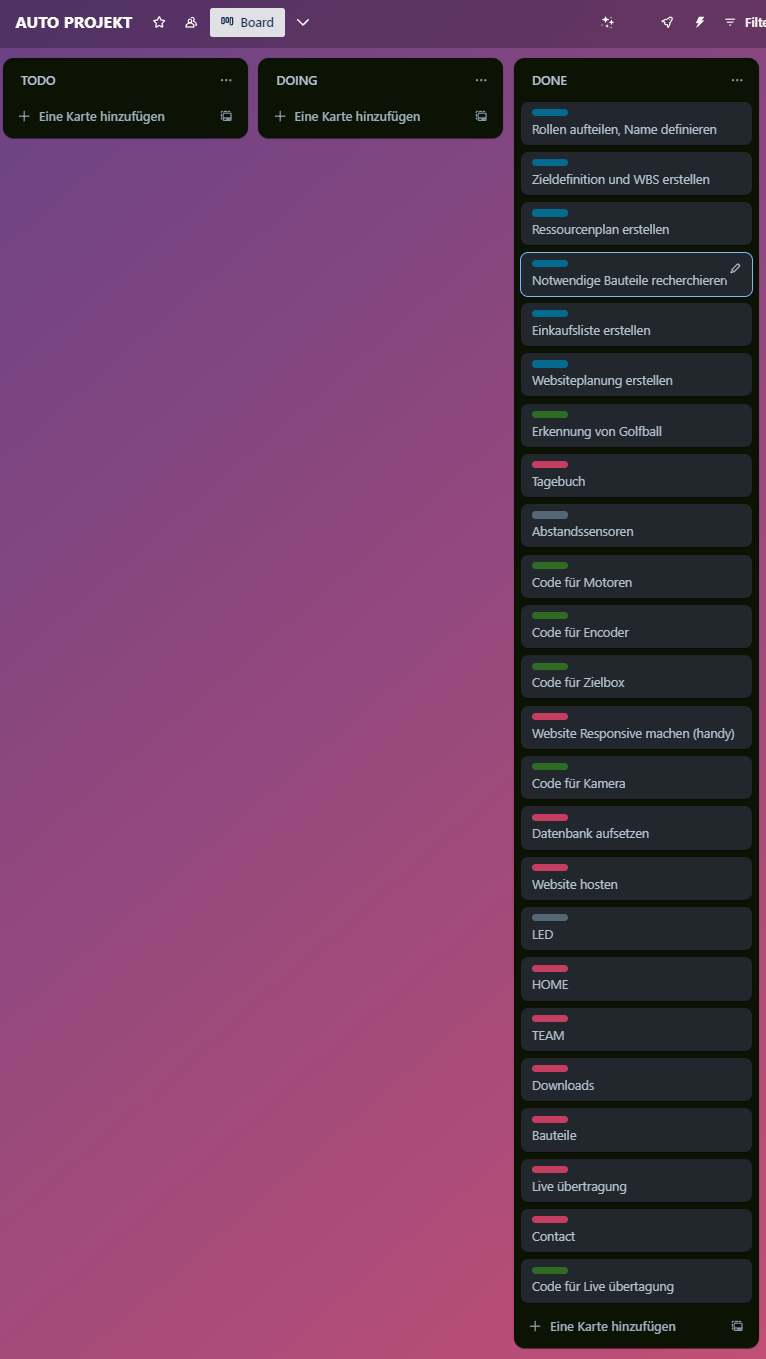
\includegraphics[width=0.85\textwidth]{Resources/kanban_board.png}
\caption{Das Kanban-Board mit farbkodierten Aufgabenbereichen.}
\end{figure}

\subsubsection{Herausforderungen und Vorteile}
Während der Nutzung von Kanban stießen wir auf einige Herausforderungen, insbesondere das gelegentliche Vergessen, Blöcke zu verschieben, was zu zeitweiligen Unklarheiten im Projektstatus führte. Trotz dieser kleinen Schwierigkeiten bot das Kanban-Board einen wertvollen Überblick über den Projektfortschritt und erlaubte es dem Team, effizient zu reagieren und Anpassungen vorzunehmen, wenn nötig.

\subsubsection{Gesamteindruck}
Die Anwendung von Kanban erwies sich als äußerst nützlich, da sie es dem Team ermöglichte, stets einen groben Überblick über den Stand des Projekts zu haben. Diese Methode förderte nicht nur die Transparenz innerhalb des Teams, sondern half auch dabei, die Projektdynamik aufrechtzuerhalten und sicherzustellen, dass alle Aufgabenbereiche angemessen adressiert wurden.
